%----------------------------------------------------------------------------------------
%	PACKAGES AND THEMES
%----------------------------------------------------------------------------------------
\documentclass[aspectratio=169,xcolor=dvipsnames, t]{beamer}
\usepackage{fontspec} % Allows using custom font. MUST be before loading the theme!
\usetheme{SimplePlusAIC}
\usepackage{hyperref}
\usepackage{graphicx} % Allows including images
\usepackage{booktabs} % Allows the use of \toprule, \midrule and  \bottomrule in tables
\usepackage{svg} %allows using svg figures
\usepackage{tikz}
\usepackage{makecell}
\usepackage{wrapfig}
\usepackage{comment}
\usepackage{animate}
\usepackage{xcolor}

\usetikzlibrary{overlay-beamer-styles}
\usetikzlibrary{shapes, positioning, calc}
\usetikzlibrary{decorations.text}
\usetikzlibrary{shapes.geometric, arrows}
% ADD YOUR PACKAGES BELOW

%----------------------------------------------------------------------------------------
%	TITLE PAGE CONFIGURATION
%----------------------------------------------------------------------------------------

\title[Section 2.3]{2.3 Scheduling jobs on identical parallel machines} % The short title appears at the bottom of every slide, the full title is only on the title page
\subtitle{CSE462: Algorithm Engineering Sessional}

\author[Samee]{Abdus Samee}
\institute[CSE462]{1805021 \newline Computer Science \& Engineering\newline Bangladesh University of Engineering  \& Technology}
% Your institution as it will appear on the bottom of every slide, maybe shorthand to save space


\date{\today} % Date, can be changed to a custom date
%----------------------------------------------------------------------------------------
%	PRESENTATION SLIDES
%----------------------------------------------------------------------------------------

\begin{document}

\maketitlepage

\begin{frame}[t]{Overview}
    % Throughout your presentation, if you choose to use \section{} and \subsection{} commands, these will automatically be printed on this slide as an overview of your presentation
    \tableofcontents
\end{frame}

%------------------------------------------------
% Section divider frame
\makesection{Introduction}

%------------------------------------------------
% Problem Definition
\begin{frame}{Problem Definition}
    \begin{itemize}
        \item \textit{m} identical machines running in parallel \pause
        \begin{itemize}
            \item Each machine can process at most $1$ job at a time \pause
        \end{itemize}
        \item \textit{n} jobs \pause
        \begin{itemize}
            \item Every job $j=1,...,n$ must be processed in one of the machines for $p_j$ time units without interruption \pause
            \item Each job is available for processing at time $0$ \pause
            \item A job $j$ completes at time $C_j$
        \end{itemize}
    \end{itemize}
\end{frame}

%------------------------------------------------
% Problem Goal
\begin{frame}{Problem Goal}
    Our goal is to complete all jobs as soon as possible \pause
    \begin{equation*}
        \text{minimize } C_{max} = max_{j=1,...,n}C_j
    \end{equation*}
    Also known as \alert{\textit{makespan}} or \alert{\textit{length}} of the schedule \pause
    \newline \newline
    Moreover, the load-balancing problem can be a similar to this, where $n$ items(or jobs) each with weight $p_j$ are distributed among $m$, in order to minimize maximum total weight assigned to one machine
\end{frame}

%------------------------------------------------
% Section divider frame
\makesection{Algorithm}

%------------------------------------------------
% Local Search
\begin{frame}{Local Search}
    \onslide<1>
    \begin{block}{What is Local Search?}
        A heuristic method which moves from one feasible solution to another optimizing a criterion defined by a set of local changes
    \end{block} \pause

    \onslide<2->
    \begin{description}
        \item[Initiation] Start with a random schedule \pause
        \item[Local move] Choose the job $j$ that finishes last \pause
        \item[Base case] Find if any machine exists to which job $j$ can be reassigned \pause
        \item[Recur or End] If a machine $m$ remains free after processing its assigned jobs before $j$ starts being processed, then we assign $j$ to $m$ and continue. Otherwise, we terminate the process
    \end{description}
\end{frame}

%------------------------------------------------
% Local Search Illustration
\begin{frame}{Local Search Illustration}
    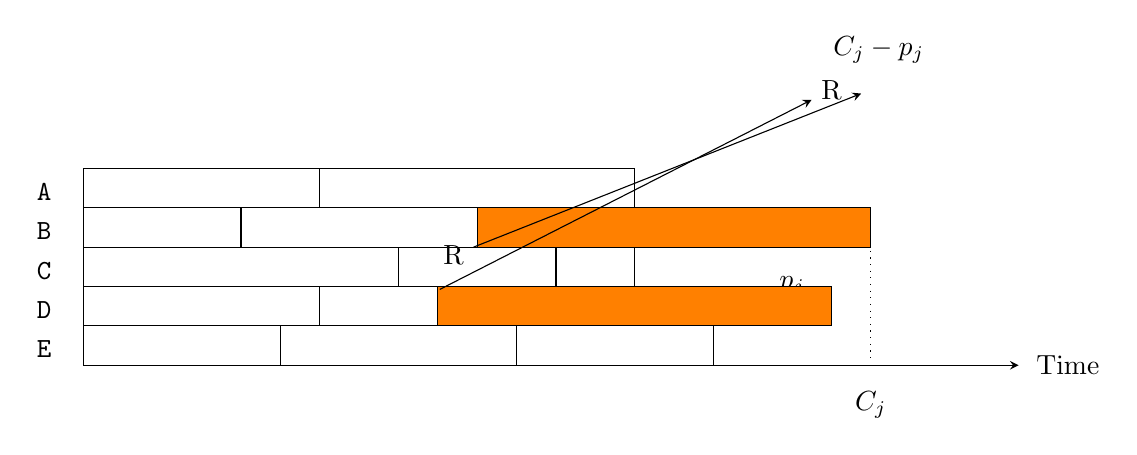
\begin{tikzpicture}
        \node (A) at (1.5,5.7) {\texttt{A}};
        \node (A) at (1.5,5.2) {\texttt{B}};
        \node (A) at (1.5,4.7) {\texttt{C}};
        \node (A) at (1.5,4.2) {\texttt{D}};
        \node (A) at (1.5,3.7) {\texttt{E}};
        
        \draw (2,5.5) rectangle (5,6);
        \draw (5,5.5) rectangle (9,6);
        \draw (2,5) rectangle (4,5.5);
        \draw (4,5) rectangle (7,5.5);
        \draw (2,4.5) rectangle (6,5);
        \draw (6,4.5) rectangle (8,5);
        \draw (8,4.5) rectangle (9,5);
        \draw (2,4) rectangle (5, 4.5);
        \draw(5,4) rectangle (6.5,4.5);
        \draw(2,3.5) rectangle (4.5,4);
        \draw(4.5,3.5) rectangle (7.5,4);
        \draw(7.5,3.5) rectangle (10,4);

        \node (a) at (7.5,3.5) {};
        \node (b) at (14,3.5) {};
        \node (c) at (14.5,3.5) {Time};
        \onslide<2> \node (d) at (12,3.4) {};
        \onslide<2> \node (dd) at (12,3) {$C_j$};
        \node (e) at (12,5.5) {};
        \onslide<2> \node (f) at (11,5.5) {};
        
        \onslide<1-> \draw[-stealth] (a) -- (b);
        \onslide<2> \draw[dotted] (e) -- (d);
        \onslide<2> \node[rectangle callout, color=black, callout relative pointer={(0,0.5)}, below of=f] {$p_j$};
        \onslide<1-3> \draw [fill=orange] (7,5) rectangle (12,5.5);

        \onslide<3> \node (g) at (6.7,4.9) {R};
        \node (h) at (12,7) {};
        \onslide<3> \node (i) at (12.1,7.5) {$C_j-p_j$};
        \onslide<3> \draw[-stealth] (g) -- (h);

        \onslide<4> \draw [fill=orange] (6.5,4) rectangle (11.5,4.5);
        \node (j) at (6.4,4.4) {};
        \node (k) at (11.5,7) {R};
        \draw[-stealth] (j) -- (k);
    \end{tikzpicture}
\end{frame}

%------------------------------------------------
% Section divider frame
\makesection{Theorem}

%------------------------------------------------
% Theoerm (in highlighted box) and Equation in text
\begin{frame}{Theorem}
    \begin{theorem}[2-approximation algorithm]
        The local search procedure for scheduling jobs on identical parallel machines is a 2-approximation algorithm
    \end{theorem}
\end{frame}

\begin{frame}{Proof}
    Suppose, \\
    The length of optimal schedule be $C_{max}^*$ \newline \newline \pause
    $x_{ij}=1$ if $i$ machine processes job $j$, otherwise $x_{ij}=0$ \newline \newline \pause
    For any machine $i$, its completion time is $\sum_{j=1}^{n} x_{ij}p_j$ \newline \newline \pause
    So,
    \begin{equation}
        C_{max}^* \ge \sum_{j=1}^{n} x_{ij}p_j
    \end{equation}
\end{frame}

%------------------------------------------------
% Figure without wrapped text
\begin{frame}{Figure}
    \begin{figure}
    \includegraphics[height=0.5\paperheight]{figures/results_fig.pdf}
    \caption{Figure caption}
    \end{figure}
\end{frame}

%------------------------------------------------
% Figure with wrapped text
\begin{frame}{Wrapped Figure}
    \begin{wrapfigure}{r}{0.4\textwidth}
    \centering
    \includegraphics[width=0.4\textwidth]{figures/results_fig.pdf}
    \caption{Figure caption}
\end{wrapfigure}
"Lorem ipsum dolor sit amet, consectetur adipiscing elit, sed do eiusmod tempor incididunt ut labore et dolore magna aliqua. Ut enim ad minim veniam, quis nostrud exercitation ullamco laboris nisi ut aliquip ex ea commodo consequat. Duis aute irure dolor in reprehenderit in voluptate velit esse cillum dolore eu fugiat nulla pariatur. Excepteur sint occaecat cupidatat non proident, sunt in culpa qui officia deserunt mollit anim id est laborum.Sed ut perspiciatis unde omnis iste natus error sit voluptatem accusantium doloremque laudantium, totam rem aperiam.
\end{frame}
%------------------------------------------------
% Section divider frame
\makesection{Citations and References}

%------------------------------------------------
% Citations
\begin{frame}[fragile] % Need to use the fragile option when verbatim is used in the slide
    \frametitle{Citation}
    An example of the \verb|\cite| command to cite within the presentation:\\~

    This statement requires citation \cite{p1}.
\end{frame}

%------------------------------------------------
% Refenrenced
\begin{frame}{References}
    % Beamer does not support BibTeX so references must be inserted manually as below
    \footnotesize{
        \begin{thebibliography}{99}
            \bibitem[Smith, 2012]{p1} John Smith (2012)
            \newblock Title of the publication
            \newblock \emph{Journal Name} 12(3), 45 -- 678.

            \bibitem[Doe, 2012]{p1} Joe Doe (2012)
            \newblock Title of the publication
            \newblock \emph{Journal Name} 12(3), 45 -- 678.
            \bibitem[Doe, 2013]{p} Jane Doe (2012)
            \newblock Title of the publication
            \newblock \emph{Journal Name} 12(3), 45 -- 678.
        \end{thebibliography}
    }
\end{frame}

%----------------------------------------------------------------------------------------
% Final PAGE
% Set the text that is showed on the final slide
\finalpagetext{Thank you for your attention}
%----------------------------------------------------------------------------------------
\makefinalpage
%----------------------------------------------------------------------------------------
\end{document}
